\documentclass[12pt]{article}

\usepackage{geometry}
\geometry{a4paper} 
\usepackage{fullpage}

\usepackage{amssymb,rotating,natbib,graphicx,fancyvrb,booktabs} 

\usepackage[parfill]{parskip} 
\usepackage[utf8]{inputenc}

\usepackage[colorlinks=true,linkcolor=blue, citecolor=blue, urlcolor=blue, linktoc=page]{hyperref}


%% double spacing
\usepackage{setspace}
 \onehalfspacing

% line numbers
% \usepackage{lineno}
% \linenumbers
% \renewcommand\linenumberfont{\normalfont\small}

%% new custom commands for code formatting
\newcommand{\code}[1]{\texttt{#1}}
\newcommand{\class}[1]{`\code{#1}'}
%\newcommand{\fct}[1]{#1}
\newcommand{\fct}[1]{\texttt{#1()}}
\newcommand{\pkg}[1]{{\fontseries{b}\selectfont #1}}
\let\proglang=\textsf

% remove page numbers
%\pagenumbering{gobble}



\title{Reproducible, flexible and high throughput data extraction from primary literature: The \pkg{metaDigitise} \proglang{R} package \vskip15pt Supplementary Materials}

\author{Joel L. Pick, Shinichi Nakagawa \& Daniel W.A. Noble}


\begin{document}


\DefineVerbatimEnvironment{Code}{Verbatim}{}
\DefineVerbatimEnvironment{CodeInput}{Verbatim}{fontshape=sl}
\DefineVerbatimEnvironment{CodeOutput}{Verbatim}{}
\newenvironment{CodeChunk}{}{}

\setcounter{equation}{0}
\setcounter{subsection}{0}

\renewcommand{\thetable}{S\arabic{table}}%
\renewcommand{\thefigure}{S\arabic{figure}}%
\renewcommand{\theequation}{S\arabic{equation}}%
\renewcommand{\thesection}{S\arabic{section}}%
\renewcommand{\thesubsection}{S\arabic{section}.\arabic{subsection}}%



\maketitle

\clearpage

\tableofcontents

\clearpage

\section{Tutorial}
\subsection{Extracting Data From Plots}
%% scatterplot from airquality data


We can demonstrate how \fct{metaDigitise} works using figures generated from the well known iris data set. \pkg{metaDigitise} can installed from GitHub as follows:

\begin{CodeChunk}
\begin{CodeInput}
R> install.packages("devtools")
R> devtools::install_github("daniel1noble/metaDigitise")
R> library(metaDigitise)
\end{CodeInput}
\end{CodeChunk}

Assume you would like to extract descriptive statistics from studies measuring sepal length or width in iris species for a fictitious project. There are a few studies that only present these data in figures. As you read papers found from a systematic search, you add figures with relevant data to a "FiguresToExtract" folder as follows

\begin{CodeChunk}
\begin{CodeOutput}
*FiguresToExtract/
    + 001_Anderson_1935_Fig1.png
\end{CodeOutput}
\end{CodeChunk}

\begin{figure}[!h]
\centering
 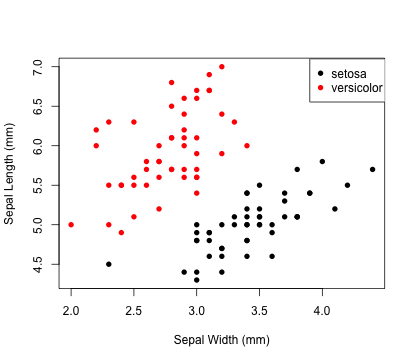
\includegraphics[width=0.75\textwidth]{001_Anderson_1935_Fig1.png} 
 \caption{Example scatterplot (001\_Anderson\_1935\_Fig1.png) of sepal length and width for two species of iris (setosa and versicolor)}
\label{fig:Anderson}
\end{figure}

Here, the naming of the files placed in the folder will contain the paper number, first author and the figure number to keep data uniquely associated with figures. At first there is one figure in the folder, shown in Figure \ref{fig:Anderson}. Running \fct{metaDigitise} brings up a series of prompts using a main menu that provides access to a number of its features ("..." here represents the user's path to the project directory): 

\begin{CodeChunk}
\begin{CodeInput}
R> digitised_data <- metaDigitise(".../FiguresToExtract", summary = TRUE)
\end{CodeInput}
\begin{CodeOutput}
	Do you want to...
1: Process new images
2: Import existing data
3: Edit existing data
Selection: 
\end{CodeOutput}
\end{CodeChunk}

You then simply enter in the numeric value that corresponds to what you would like to do. In this case we want to "Process new images". You are then asked whether there are different types of plot(s) in the folder. This question is most relevant when there are lots of different figures in the folder because it will then ask for the type of figure as they are cycled through.

\begin{CodeChunk}
\begin{CodeOutput}
Are all plot types Different or the Same? (d/s)
\end{CodeOutput}
\end{CodeChunk}

\fct{metaDigitise} then asks whether the figure needs to be rotated or flipped. This can be needed when box plots and mean and error plots are not orientated correctly. In some cases, older papers can give slightly off angled images which can be corrected by rotating. In this prompt the user has three options: \code{f} for ``Flip'', \code{r} for ``rotate'' or \code{c} for ``continue''. 

\begin{CodeChunk}
\begin{CodeOutput}
mean_error and boxplots should be vertically orientated
       _ 
       |  
  I.E. o    NOT  |-o-|
       |
       _

If they are not then chose flip to correct this.

If figures are wonky, chose rotate.

Otherwise chose continue

Flip, rotate or continue (f/r/c) 
\end{CodeOutput}
\begin{CodeInput}
R> c
\end{CodeInput}
\end{CodeChunk}

After this, \fct{metaDigitise} will ask you to specify the plot type. Depending on the figure, you can specify that it is a figure containing the mean and error (\code{m}), a box plot (\code{b}), a scatter plot (\code{s}) or a histogram (\code{h}). If you has specified \code{d} instead of \code{s} in response to the question about whether the plot types are the same or different, this question will pop up for each plot, but will only be asked once if plots are all the same.

\begin{CodeChunk}
\begin{CodeOutput}
Please specify the plot_type as either:

 m: Mean and error
 b: Box plot
 s: Scatter plot 
 h: Histogram
\end{CodeOutput}
\begin{CodeInput}
R> s
\end{CodeInput}
\end{CodeChunk}

After selecting the figure type a new set of prompts will come up that will ask what the y and x-axis variables are. This is useful as users can keep track of the different variables across figures and papers. Here, you can just add this information in to the \proglang{R} console. Once complete, details on how to calibrate the x and y-axis appear, so that the relevant statistics / data can be correctly calculated. When working with a plot of mean and errors, the x-axis is rather useless in terms of calibration so \fct{metaDigitise} just asks you to calibrate the y-axis. 

\begin{CodeChunk}
\begin{CodeOutput}
What is the y variable? 
\end{CodeOutput}
\begin{CodeInput}
R> Sepal Length (mm)
\end{CodeInput}

\begin{CodeOutput}
What is the x variable? 
\end{CodeOutput}
\begin{CodeInput}
R> Sepal Width (mm)
\end{CodeInput}

\begin{CodeOutput}
On the Figure, click IN ORDER: 
      y1, y2 , x1, x2  


    Step 1 ----> Click on known value on y axis - y1
  |
  |
  |
  |
  y1
  |_________________________
  ....

    Step 3 ----> Click on known value on x axis - x1
  |
  |
  |
  |
  |
  |_____x1__________________

  ....
\end{CodeOutput}
\end{CodeChunk}

You can just follow the instructions on screen step-by-step (instructions above have been truncated by `...' to simplify), and in the order specified. Before moving on, you are forced to check whether or not the calibration has been set up correctly. If \code{n} is chosen because something needs to be fixed then you can re-calibrate.

\begin{CodeChunk}
\begin{CodeOutput}
What is the value of y1 ?
\end{CodeOutput}
\begin{CodeInput}
R> 4.5
\end{CodeInput}
\begin{CodeOutput}
What is the value of y2 ?
\end{CodeOutput}
\begin{CodeInput}
R> 7
\end{CodeInput}
\begin{CodeOutput}
What is the value of x1 ?
\end{CodeOutput}
\begin{CodeInput}
R> 2
\end{CodeInput}
\begin{CodeOutput}
What is the value of x2 ?
\end{CodeOutput}
\begin{CodeInput}
R> 4
\end{CodeInput}
\begin{CodeOutput}
Re-calibrate? (y/n) 
\end{CodeOutput}
\begin{CodeInput}
R> n
\end{CodeInput}
\end{CodeChunk}

Often, plots might contain multiple groups that a meta-analyst wants to extract from. \fct{metaDigitise} handles this nicely by prompting you to enter the group first, followed by digitisation of this groups data. After digitising the first group, \fct{metaDigitise} will ask whether you would like to add another group. You can continually add groups (\code{a}), delete groups (\code{d}), edit groups (\code{e}) or finish a plot and continue to the next one (\code{f} - if another plot exists). 
%%% This needs checking - think it is now different
The number of groups are not really limited and you can just keep adding in groups to accommodate the different numbers that may be presented across figures (although it can get complicated with too many).

\begin{CodeChunk}
\begin{CodeOutput}
If there are multiple groups, enter unique group identifiers (otherwise press enter)
Group identifier: 
\end{CodeOutput}
\begin{CodeInput}
R> setosa
\end{CodeInput}
\begin{CodeOutput}
Click on points you want to add.
If you want to remove a point, or are finished with a group, 
exit by clicking on red box in bottom left corner, then follow prompts
\end{CodeOutput}
\end{CodeChunk}

To finish selecting points, you can exit by clicking on the red button that appears when extracting points. You are then asked if you want to add or delete points from that group. 

\begin{CodeChunk}
\begin{CodeOutput}
Add or Delete points to this group, or Continue? (a/d/c) 
\end{CodeOutput}
\begin{CodeInput}
R> c
\end{CodeInput}
\end{CodeChunk}

Once we are done digitising all the groups our plot will look something like Figure \ref{fig:scatter_extract}.

\begin{figure}[!h] 
\centering
 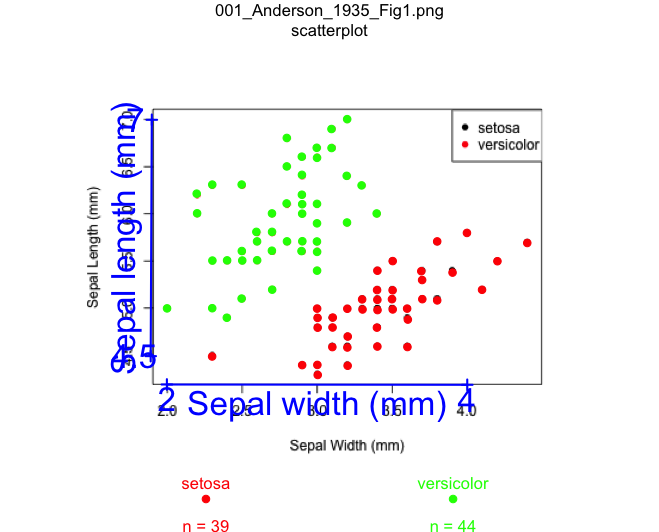
\includegraphics[width=0.75\textwidth]{001_Anderson_1935_Fig1_digitised.png} 
 \caption{Digitisation of sepal length and width for two species of iris (setosa and versicolor). Names of the variables and calibration (in blue) are plotted alongside the digitised points (green = versicolor; red = setosa). The sample sizes for each group are provided on the lower part of the plot. All figures are clearly labelled at the top to remind users of the filename and plot type. This reduces errors throughout the digitisation process.}
\label{fig:scatter_extract}
\end{figure}

When completed \fct{metaDigitise} will write the digitised data as a \code{metaDigitise} object to a RDS file in the caldat directory, such that our new directory structure is as follows

\begin{CodeChunk}
\begin{CodeOutput}
*FiguresToExtract/
    + caldat/
        + 001_Anderson_1935_Fig1
    + 001_Anderson_1935_Fig1.png
\end{CodeOutput}
\end{CodeChunk}

You can access the \code{metaDigitise} object created (001\_Anderson\_1935\_Fig1) at any time using the \fct{metaDigitse} function. In the \proglang{R} console, the summarised data for the digitised figure can be printed on screen or even written to a .csv file:

\begin{CodeChunk}
\begin{CodeInput}
R> digitised_data
\end{CodeInput}
{\scriptsize
\begin{CodeOutput}
                  filename    group_id         variable  mean  error error_type  n     r    sd  plot_type
001_Anderson_1935_Fig1.png      setosa  Sepal width (mm)  3.42  0.40  sd        39  0.75  0.40  scatterplot
001_Anderson_1935_Fig1.png      setosa  Sepal length (mm) 5.00  0.38  sd        39  0.75  0.38  scatterplot
001_Anderson_1935_Fig1.png  versicolor  Sepal width (mm)  2.77  0.32  sd        44  0.52  0.32  scatterplot
001_Anderson_1935_Fig1.png  versicolor  Sepal length (mm) 5.95  0.53  sd        44  0.52  0.53  scatterplot
\end{CodeOutput}
}
\end{CodeChunk}

The mean for each of the two variables, along with the two species, are provided. Since this is a scatterplot, the user also gets the Person's correlation coefficient between sepal length and width for each species. These match reasonably well with the actual means of sepal length and width for each of the species in the full `iris` dataset:

\begin{CodeChunk}
\begin{CodeOutput}
     Species meanSL meanSW
1     setosa  5.006  3.428
2 versicolor  5.936  2.770
\end{CodeOutput}
\end{CodeChunk}

One thing anyone with a familiarity with the iris dataset will notice is that the sample sizes for each of these species (which are n = 50 each) are quite a bit lower. This is an example of some of the challenges when extracting data from scatter plots. Often data points will overlap with each other making it impossible (without having the real data) to know whether this is a problem. However, a meta-analyst will probably realise that the sample sizes here conflict with what is reported in the paper. Hence, \pkg{metaDigitise} also provides you with  options to input the sample sizes directly, even for scatter plots and histograms where, strictly speaking, this should not be necessary. Nonetheless, it is important to recognise the impact that overlapping points can have on summary statistics, particularly its effects on sampling variance. Here, the mean point estimates are nearly exactly the same as the true values, but the SD's are slightly over-estimated:

\begin{CodeChunk}
\begin{CodeOutput}
     Species    meanSL    meanSW
1     setosa 0.3524897 0.3790644
2 versicolor 0.5161711 0.3137983
\end{CodeOutput}
\end{CodeChunk}



\subsection{Adding new figures}

You can add additional figures to the directory as new papers with relevant information are found. Each figure should be in its own file with unique naming, even if a single paper has multiple figures for extraction. For example, another paper on different populations (and one new species) of iris contained two additional figures where important data could be extracted. These figures can simply be named accordingly and added directly to the same extraction folder: 

\begin{CodeChunk}
\begin{CodeOutput}
*FiguresToExtract/
    + caldat/
        + 001_Anderson_1935_Fig1
    + 001_Anderson_1935_Fig1.png
    + 002_Doe_2013_Fig1.png
    + 002_Doe_2013_Fig3.png
\end{CodeOutput}
\end{CodeChunk}

We have already processed one figure (001\_Anderson\_1935\_Fig1.png). We can tell this because the caldat folder has digitised data in it (caldat/001\_Anderson\_1935\_Fig1). Now there are two new figures that have not yet been digitised. This example will also nicely demonstrate how you can easily pick up from where you left off and how previous data gets re-integrated. It will also demonstrate how different plot types are handled. All we have to do to begin, is again, provide the directory where all the figures are located:

\begin{CodeChunk}
\begin{CodeInput}
R> digitised_data <- metaDigitise("~/FiguresToExtract", summary = TRUE)
\end{CodeInput}
\end{CodeChunk}

You get the same set of prompts and simply chooses option one. This will permit users to digitise new figures, and will integrate previously completed digitisations along with newly digitised data together at the end of the session, or when the you decides to quit. This time, 001\_Anderson\_1935\_Fig1.png is ignored and the new plots cycle on screen; first 002\_Doe\_2013\_Fig1.png and then 002\_Doe\_2013\_Fig3.png. Since there are a few different figure types, you answer the first question in the \proglang{R} console as "d":

\begin{CodeChunk}
\begin{CodeOutput}
Are all plot types Different or the Same? (d/s)
\end{CodeOutput}
\begin{CodeInput}
R> d
\end{CodeInput}
\begin{CodeOutput}
**** NEW PLOT ****

mean_error and boxplots should be vertically orientated
       _ 
       |  
  I.E. o    NOT  |-o-|
       |
       _

If they are not then chose flip to correct this.

If figures are wonky, chose rotate.

Otherwise chose continue

Flip, rotate or continue (f/r/c) 
\end{CodeOutput}
\begin{CodeInput}
R> c
\end{CodeInput}
\begin{CodeOutput}
Please specify the plot_type as either:

 m: Mean and error
 b: Box plot
 s: Scatter plot 
 h: Histogram
\end{CodeOutput}
\begin{CodeInput}
R> m
\end{CodeInput}
\end{CodeChunk}

Here, you specify the new plot type as \code{m} for 002\_Doe\_2013\_Fig1.png because this a plot of the mean and error of sepal length for each of the three species. The user is then prompted a bit differently from our scatter plot as the x-axis is not needed for calibration:

\begin{CodeChunk}
\begin{CodeOutput}
What is the y variable? 
\end{CodeOutput}
\begin{CodeInput}
R> Sepal length
\end{CodeInput}
\begin{CodeOutput}
On the Figure, click IN ORDER: 
      y1, y2  


    Step 1 ----> Click on y1
  |
  |
  |
  |
  y1
  |_________________________


    Step 2 ----> Click on y2
  |
  y2
  |
  |
  |
  |_________________________
  
What is the value of y1 ?
\end{CodeOutput}
\begin{CodeInput}
R> 5
\end{CodeInput}
\begin{CodeOutput}
What is the value of y2 ?
\end{CodeOutput}
\begin{CodeInput}
R> 6.5
\end{CodeInput}
\begin{CodeOutput}
Re-calibrate? (y/n) 
\end{CodeOutput}
\begin{CodeInput}
R> n
\end{CodeInput}
\begin{CodeOutput}
Do you know sample sizes? (y/n)  
\end{CodeOutput}
\begin{CodeInput}
R> y
\end{CodeInput}
\begin{CodeOutput}
If there are multiple groups, enter unique group identifiers (otherwise press enter)
Group identifier: 
\end{CodeOutput}
\begin{CodeInput}
R> setosa
\end{CodeInput}
\begin{CodeOutput}
Group sample size: 
\end{CodeOutput}
\begin{CodeInput}
R> 50
\end{CodeInput}
\begin{CodeOutput}
Click on Error Bar, followed by the Mean

Add group, Edit Group, Delete group or Finish plot? (a/e/d/f) 
\end{CodeOutput}
\begin{CodeInput}
R> a
\end{CodeInput}
\end{CodeChunk}

Again, \fct{metaDigitise} will simply guide you through digitising each of these figures describing to you exactly what needs to be done. At any point if mistakes are made you can choose relevant options to edit or correct things before ending the figure. This process continues for each plot so long as the you would like to continue and after completing a single plot you are always prompted as follows:

\begin{CodeChunk}
\begin{CodeOutput}
Do you want continue: 1 plots out of 2 plots remaining (y/n)
\end{CodeOutput}
\begin{CodeInput}
R> y
\end{CodeInput}
\end{CodeChunk}

This continues until you have completed all non-digitised figures in the folder, at which point \fct{metaDigitise} concatenates the new data with previously digitised data in the object:

\begin{CodeChunk}
{\scriptsize
\begin{CodeOutput}
data
                  filename    group_id         variable   mean  error error_type n    r    sd   plot_type
001_Anderson_1935_Fig1.png      setosa  Sepal width (mm)  3.42  0.40  sd        39  0.75  0.40  scatterplot
001_Anderson_1935_Fig1.png      setosa  Sepal length (mm) 5.00  0.38  sd        39  0.75  0.38  scatterplot
001_Anderson_1935_Fig1.png  versicolor  Sepal width (mm)  2.77  0.32  sd        44  0.52  0.32  scatterplot
001_Anderson_1935_Fig1.png  versicolor  Sepal length (mm) 5.95  0.53  sd        44  0.52  0.53  scatterplot
     002_Doe_2013_Fig1.png      setosa  Sepal length      5.00  0.11  se        50  NA    0.78  mean_error
     002_Doe_2013_Fig1.png  viriginica  Sepal length      6.59  0.18  se        50  NA    1.26  mean_error
     002_Doe_2013_Fig1.png  versicolor  Sepal length      5.94  0.14  se        50  NA    1.01  mean_error
     003_Doe_2013_Fig3.png      catana  Sepal length      4.95  0.36  sd        50  NA    0.36  histogram
\end{CodeOutput}
}
\end{CodeChunk}


\subsection{Re-importing, Editing and Plotting Previously Digitised data}

A particularly useful feature of \pkg{metaDigitise} is its ability to re-import, edit and re-plot previously digitised figures. We can do this from the initial options from \fct{metaDigitise}


\begin{CodeChunk}
\begin{CodeInput}
R> digitised_data <- metaDigitise(".../FiguresToExtract")
\end{CodeInput}
\begin{CodeOutput}
    Do you want to...
1: Process new images
2: Import existing data
3: Edit existing data
Selection: 
\end{CodeOutput}
\end{CodeChunk}

If we choose "Import existing data", you have the option of either 1) importing data from all digitised images or 2) importing data from a single image that has been digitised. If 2, then a list of files are provided for you to select. Editing existing data allows you to easily re-plot or edit information or digitisations that have previously be done for any plot. This is accomplished by guiding you through a new set of options:

\begin{CodeChunk}
\begin{CodeOutput}
Choose how you want to edit files:
1: Cycle through images
2: Choose specific file to edit
3: Enter previously omitted sample sizes
Selection: 
\end{CodeOutput}
\end{CodeChunk}

If you is unsure about the name of the specific figure you need to edit or simply want to just check the digitisations of figures they can choose "Cycle through images", which will bring up each figure, one by one, overlaying the calibrations, group names (if they exist), sample sizes (if they were entered) and the selected points. The user will then be given the choice to edit individual images. Alternatively, choosing option 2, will bring up a list of the completed files in the folder and the specific file can be chosen, at which point it will be replotted. Either of these options will cycle through a number of questions asking you what they would like to edit:

\begin{CodeChunk}

\begin{CodeOutput}
Edit rotation? If yes, then the whole extraction will be redone (y/n) 
\end{CodeOutput}
\begin{CodeInput}
R> n
\end{CodeInput}
\begin{CodeOutput}
Change plot type? If yes, then the whole extraction will be redone (y/n) 
\end{CodeOutput}
\begin{CodeInput}
R> n
\end{CodeInput}
\begin{CodeOutput}
Variable entered as: 
Sepal length
Rename Variables (y/n) 
\end{CodeOutput}
\begin{CodeInput}
R> n
\end{CodeInput}
\begin{CodeOutput}
Edit calibration? (y/n) 
\end{CodeOutput}
\begin{CodeInput}
R> n
\end{CodeInput}
\begin{CodeOutput}
Re-extract data (y/n) 
\end{CodeOutput}
\begin{CodeInput}
R> y
\end{CodeInput}
\begin{CodeOutput}
Change group identifier? (y/n) 
\end{CodeOutput}
\begin{CodeInput}
R> n
\end{CodeInput}
\begin{CodeOutput}
Add group, Delete group or Finish plot? (a/d/f) 
\end{CodeOutput}
\begin{CodeInput}
R> d
\end{CodeInput}
\begin{CodeOutput}
1: setosa
2: versicolor
3: viriginica
Selection: 
\end{CodeOutput}
\begin{CodeInput}
R> 2
\end{CodeInput}
\begin{CodeOutput}
Add group, Delete group or Finish plot? (a/d/f) 
\end{CodeOutput}
\begin{CodeInput}
R> a
\end{CodeInput}

\end{CodeChunk}

A whole host of information can be edited including the rotation, plot type, the variable name(s) that were provided, the calibration and even the digitisation of groups. When editing the \code{metaDigitise} object is re-written to the caldat folder and the edits are immediately integrated into the existing object once complete. 

\subsection{Obtaining Calibrated Data}

While \fct{metaDigitise} provides you with the summary statistics by default, for all plot types, in many cases the user may actually be interested in obtaining the calibrated data from scatter plots (i.e. all calibrated points). This is very easy to do by changing the default \code{summary} argument from TRUE to FALSE in \fct{metaDigitise}. Instead of providing you with summary statistics it will return a list containing four slots for each of the figure types (mean error, box plot, histogram and scatter plots). An example of a data object returned from digitising figures is as follows:

\begin{CodeChunk}

\begin{CodeInput}
>R str(data)
\end{CodeInput}

\begin{CodeOutput}
List of 3
 $ mean_error :List of 1
  ..$ 002_Doe_2013_Fig1.png:'data.frame': 3 obs. of  5 variables:
  .. ..$ id      : Factor w/ 3 levels "setosa","versicolor",..: 1 2 3
  .. ..$ mean    : num [1:3] 5 5.93 6.59
  .. ..$ error   : num [1:3] 0.111 0.148 0.178
  .. ..$ n       : num [1:3] 50 50 50
  .. ..$ variable: chr [1:3] "Sepal length" "Sepal length" "Sepal length"
 $ hist       :List of 1
  ..$ 003_Doe_2013_Fig3.png:'data.frame': 8 obs. of  3 variables:
  .. ..$ midpoints: num [1:8] 4.3 4.5 4.7 4.9 5.1 ...
  .. ..$ frequency: num [1:8] 4 5 7 12 11 6 2 3
  .. ..$ variable : chr [1:8] "Sepal length" "Sepal length" ...
 $ scatterplot:List of 1
  ..$ 001_Anderson_1935_Fig1.png:'data.frame':  83 obs. of  8 variables:
  .. ..$ id        : Factor w/ 2 levels "setosa","versicolor": 1 1 1 1 1 ...
  .. ..$ x         : num [1:83] 2.3 2.9 3 3 3 ...
  .. ..$ y         : num [1:83] 4.5 4.4 4.41 4.3 4.8 ...
  .. ..$ group     : num [1:83] 1 1 1 1 1 1 1 1 1 1 ...
  .. ..$ col       : Factor w/ 2 levels "red","green": 1 1 1 1 1 1 1 1 1 ...
  .. ..$ pch       : num [1:83] 19 19 19 19 19 19 19 19 19 19 ...
  .. ..$ y_variable: chr [1:83] "Sepal length (mm)" "Sepal length (mm)"  ...
  .. ..$ x_variable: chr [1:83] "Sepal width (mm)" "Sepal width (mm)"    ...
\end{CodeOutput}
\end{CodeChunk}

Here, the user can easily access the list of calibrated scatter plot data by simply extracting the scatter plot slot:

\begin{CodeChunk}
\begin{CodeInput}
>R scatterplot <- data$scatterplot
\end{CodeInput}
\end{CodeChunk}


Additionally there is another function, \fct{getExtracted}, that imports all digitised data from a directory, as either summarised or calibrated data. For example,

\begin{CodeChunk}
\begin{CodeInput}
>R getExtracted(".../FiguresToExtract", summary=TRUE)
\end{CodeInput}
{\scriptsize
\begin{CodeOutput}
                  filename    group_id         variable   mean  error error_type n    r    sd   plot_type
001_Anderson_1935_Fig1.png      setosa  Sepal width (mm)  3.42  0.40  sd        39  0.75  0.40  scatterplot
001_Anderson_1935_Fig1.png      setosa  Sepal length (mm) 5.00  0.38  sd        39  0.75  0.38  scatterplot
001_Anderson_1935_Fig1.png  versicolor  Sepal width (mm)  2.77  0.32  sd        44  0.52  0.32  scatterplot
001_Anderson_1935_Fig1.png  versicolor  Sepal length (mm) 5.95  0.53  sd        44  0.52  0.53  scatterplot
     002_Doe_2013_Fig1.png      setosa  Sepal length      5.00  0.11  se        50  NA    0.78  mean_error
     002_Doe_2013_Fig1.png  viriginica  Sepal length      6.59  0.18  se        50  NA    1.26  mean_error
     002_Doe_2013_Fig1.png  versicolor  Sepal length      5.94  0.14  se        50  NA    1.01  mean_error
     003_Doe_2013_Fig3.png      catana  Sepal length      4.95  0.36  sd        50  NA    0.36  histogram
\end{CodeOutput}
}
\end{CodeChunk}

This function is useful in scripts the extracted data simply needs to be imported, and where the interactive element of \fct{metaDigitise} becomes problematic.

\subsection{Adding sample sizes to previous Digitisations}
%Including addition of N later
In many cases important information, such as sample sizes, may not be readily available or clear when digitising figures. In these circumstances you would have answered `no' to the question about whether you have sample sizes or not while digitising. To expedite finding and adding in these sample sizes to do the necessary calculations (if for example a figure presented 95\% CI's or standard errors), \fct{metaDigitise} has s specific edit option that allows users to enter in previously omitted sample sizes. It works by first identifying the missing sample sizes in the digitised output, re-plotting the relevant figure and then prompting you to enter the sample sizes for the relevant groups in the figure, one by one. As an example, assume that we were missing sample sizes for two groups in 002\_Doe\_2013\_Fig1.png:

\begin{CodeChunk}
{\scriptsize
\begin{CodeOutput}
            filename    group_id         variable   mean  error error_type n    r    sd   plot_type
002_Doe_2013_Fig1.png      setosa  Sepal length      5.00  0.11  se        NA  NA    NA  mean_error
002_Doe_2013_Fig1.png  viriginica  Sepal length      6.59  0.18  se        NA  NA    NA  mean_error
\end{CodeOutput}
}
\end{CodeChunk}

Here, we can see that we are missing the sample sizes for setosa and viriginica, and as a result, sd is not calculated because \fct{metaDigitise} needs this information to make the calculation. If, for examnple, you found this information after contacting the authors for clarification then you can add these in as follows:

\begin{CodeChunk}
\begin{CodeInput}
R> digitised_data <- metaDigitise(".../FiguresToExtract")
\end{CodeInput}
\end{CodeChunk}

\begin{CodeChunk}
\begin{CodeOutput}
Do you want to...

1: Process new images
2: Import existing data
3: Edit existing data

Selection:
\end{CodeOutput}
\begin{CodeInput}
R> 3
\end{CodeInput}
\end{CodeChunk}

\begin{CodeChunk}
\begin{CodeOutput}
Choose how you want to edit files:

1: Cycle through images
2: Choose specific file to edit
3: Enter previously omitted sample sizes

Selection:
\end{CodeOutput}
\begin{CodeInput}
>R 3
\end{CodeInput}
\end{CodeChunk}

\fct{metaDigitise} will replot the figure after this and list, only the groups missing data, for which you can then update the data. This is then re-integrated back into the data automatically and the sd calculated. 

\begin{CodeChunk}
\begin{CodeOutput}
Group " setosa ": Enter sample size  
\end{CodeOutput}
\begin{CodeInput}
R> 50
\end{CodeInput}
\begin{CodeOutput}
Group " viriginica ": Enter sample size
\end{CodeOutput}
\begin{CodeInput}
R> 50
\end{CodeInput}
\end{CodeChunk}


\clearpage

\section{Derivation of mean, standard deviation and sample size from different plot types}

\subsection{Mean/Error Plots}
The standard deviation is calculated depending on the type of error presented. The user can choose from standard deviation (SD, $\sigma$), standard error (SE) or 95\% confidence intervals (CI95). Standard deviation is calculated from standard error as
\begin{equation}
\sigma = SE \sqrt{n}
\end{equation}
and from 95\% confidence intervals as
\begin{equation}
\sigma = \frac{CI}{1.96} \sqrt{n}
\end{equation}

\subsection{Box Plots} 
The mean ($\mu$) and SD are calculated sing the maximum ($b$), upper quartile ($q_3$), median ($m$), lower quartile ($q_1$) and minimum ($a$) as 
\begin{equation}
\mu = \frac{(n+3)(a+b) + 2(n-1)(q_1 + m + q_3)}{8n}
\end{equation}
following \citet{Bland2015} and
\begin{equation}
\sigma = \frac{b-a}{4\Phi^{-1}(\frac{n-0.375}{n+0.25})} + \frac{q_3-q_1}{4\Phi^{-1}(\frac{0.75n-0.125}{n+0.25})}
\end{equation}
where $\Phi^{-1}(z)$ is the upper zth percentile of the standard normal distribution, following \citet{Wan2014}. 

\subsection{Histograms} 
For each bar, the user click two point (the top of the bar). Using these points, a midpoint (m; mean x coordinates) and a frequency (f; mean y coordinates, rounded to the nearest integer) is calculated for each bar. The sample size, mean and SD are calculated as:
\begin{equation}
n = \sum_{i=1}^n{f_i}
\end{equation}

\begin{equation}
\mu = \frac{\sum_{i=1}^n{m_i f_i}}{n}
\end{equation}

\begin{equation}
\sigma = \sqrt{\frac{\sum_{i=1}^n{(m_i f_i - \mu f_i)^2}}{n-1}}
\end{equation}


\clearpage

\section{Software Validation: Details of Simulations}

\subsection{Inter-observer variability in digitisations}
In order to evaluate the consistency of digitisation using \pkg{metaDigitise} between users, we simulated a dataset of two variables with two groups ($n=10$ within groups). Each variable was plotted twice for each plot type (figures were modified slightly to give users a sense that they were digitising new data) generating a total of 14 figures. Fourteen independent digitisers (including the authors) were provided with a directory with all 14 figures in a randomised order. Digitisers ran \pkg{metaDigistise} on their own computers, across different operating systems (including Mac, Windows and Linux). Digitisers varied in their level of experience, from people with experience of meta-analyses to those without any science background. We asked users to digitise all 14 figures and collected the mean, standard deviation and correlation coefficient ($r$, for scatter plots) generated by \fct{metaDigitise} for every plot digitised ($n=28$ per digitiser per metric, $n=4$ for $r$). 

As a measure of bias, we calculated the percentage differences from the true summary statistics as

\begin{equation}
\frac{\theta - \hat{\theta}}{\hat{\theta}}
\end{equation}

where $\theta$ is the estimate and $\hat{\theta}$ is the true value. The deviation from the true value of $r$ was not further standardised, as it is already on a standardised scale. We also took the absolute values of these standardised differences as a measure of precision. The resulting data was used to assess between- and within- user variability (i.e., the intra-class correlation coefficient - ICC). This was done using linear mixed effect models with user identity as a random effect using \pkg{lme4} \citep{bates2015} in \proglang{R}. Standardised mean, standard deviation and correlation coefficients were used as response variables in separate models. Sampling variance for ICC estimates was generated based on 1000 parametric bootstraps of the model and the significance was tested using likelihood ratio tests, using \pkg{rptR} \citep{stoffel2017}.  


\subsection{Testing the accuracy of digitisations}
To test how accurate \pkg{metaDigitise} is at matching clicked points to their true values, we generated four random scatterplots, each with 20 data points, and digitised these with \fct{metaDigitise}. This was done by one digitiser (J.L.P.), as there is no detectable between user variation.


\clearpage

\section{Comparison with existing software}
\begin{table}[h!]
\centering
\rotatebox{90}{%
\begin{minipage}{1.35\textwidth}
\small
\begin{tabular}{lccccccc}
\hline
Function                  & metaDigitise & GraphClick$^1$ & DataThief$^2$  & DigitizeIt$^3$ & WebPlotDigitizer$^4$ & metagear$^5$ & digitize$^6$\\
\hline
Scatterplots              & \checkmark   & \checkmark & \checkmark & \checkmark & \checkmark     & \checkmark$^7$ & \checkmark \\
Mean/error plots      & \checkmark   & \checkmark & \checkmark & $\times$   & $\times$       & \checkmark$^7$ & $\times$    \\
Boxplots                  & \checkmark   & $\times$   & $\times$   & $\times$   & $\times$       & $\times$       & $\times$    \\
Histograms                & \checkmark   & $\times$   & $\times$   & $\times$   & \checkmark$^7$ & $\times$       & $\times$    \\
Graph rotation$^8$        & \checkmark   & \checkmark & \checkmark & \checkmark & \checkmark     & $\times$       & $\times$    \\
Groups                    & \checkmark   & \checkmark & $\times$   & \checkmark & \checkmark     & $\times$       & $\times$    \\
Entry of metadata         & \checkmark   & $\times$   & $\times$   & $\times$   & $\times$       & $\times$       & $\times$    \\
Summarising data          & \checkmark   & $\times$   & $\times$   & $\times$   & $\times$       & $\times$       & $\times$    \\
Multiple image processing & \checkmark   & $\times$   & $\times$   & $\times$   & $\times$       & $\times$       & $\times$    \\
Reproducable$^9$  & \checkmark   & \checkmark & \checkmark & $\times$   & \checkmark     & $\times$       & $\times$    \\
Automated point detection & $\times$     & \checkmark &     $\times$      & \checkmark & \checkmark     & \checkmark     & $\times$    \\
Line extraction           & $\times$     & \checkmark & \checkmark & \checkmark & \checkmark     & $\times$       & $\times$    \\
Zoom                      & $\times$     & \checkmark & \checkmark & \checkmark & \checkmark     & $\times$       & $\times$    \\
Log axis                  & $\times$   & \checkmark & \checkmark & \checkmark & \checkmark     & $\times$       & $\times$    \\
Dates                     & $\times$   & $\times$   & \checkmark & $\times$   & \checkmark     & $\times$       & $\times$    \\
Asymmetric error bars     & $\times$     & $\times$   & \checkmark & $\times$   & $\times$       & $\times$       & $\times$    \\
Freeware                  & \checkmark$^{10}$ & \checkmark$^{11}$ & \checkmark$^{11}$ & $\times$$^{11}$ & \checkmark$^{11}$ & \checkmark$^{10}$ & \checkmark$^{10}$\\
\hline

%http://datathief.org/DatathiefManual.pdf
%http://www.digitizeit.de/#Features
%https://automeris.io/WebPlotDigitizer/userManual.pdf

\end{tabular}
\\
$^1$ \citet{GraphClick}
$^2$ \citet{DataThief}
$^3$ \citet{DigitizeIt}
$^4$ \citet{WebPlotDigitizer}
$^5$ \citet{Lajeunesse2016}
$^6$ \citet{Poisot2011}
\\$^7$ Only automated, no manual extraction.
\\$^8$ Or handles rotated graphs. 
\\$^9$ Allows saving, re-plotting and editing of data extraction.
\\$^{10}$ \proglang{R} package.
\\$^{11}$ Standalone software.
\caption{\label{tab:comparison} Comparison of functionality between different digitisation softwares.}
\end{minipage}
}

 
\end{table}

\clearpage


\bibliographystyle{FuncEcol.bst}
\bibliography{metaDigitise}


\end{document}


